\subsubsection{Minuta de reunião (05-Novembro-2015)}

\begin{tabbing}
  Local \= xxx \kill
  Local \> : LEAD \\
  Data  \> : 05 de Novembro de 2015 \\
  Hora  \> : 13:00
\end{tabbing} 

%---------------------------------------------------------------------
\participantes{
  \gabriel,
  \julia,
  \estevão,
  \elael,
  \renan,
  \ramon.

}

\textbf{Aprovação da minuta}

\textbf{Update semanal do Projeto EMMA}
   									
						
\textbf{\gabriel.} 
	\begin{itemize}
			\item Iniciou o processo de compras para Sensor de scaneamento de
			ambiente.
			\item Estudo sobre localização de objetos com PCL. Encontrou Dataset com
			modelos compatíveis.
			\end{itemize}
		
		\item \textbf{Novas tarefas:}
			\begin{itemize} 
				\item Estudo sobre 'welding'. Laboratórios na UFRJ que façam pesquisa na
				área.
				\item Teste utilizando imagem de 'point cloud' gerada pelo sensor da Faro
				durante o teste em Jirau.
			\end{itemize}

					
			
   \textbf{\estevão.} 
	\begin{itemize}
		\item \textbf{Tarefas concluídas:}
			\begin{itemize}    
			    \item Desenho do último conceito de base proposto.
				\item Orçamento do Motoman, perguntas de volta aos fornecedores.
				\item Maquete 1:1 com professor da UFRJ.
				
			\end{itemize}
		
		\item \textbf{Novas tarefas:}
			\begin{itemize} 
			    \item Formalizar último conceito de base.
			    \item Repassar possibilidadepara customização do Modelo de Motoman que
			    queremos.
			\end{itemize}
	\end{itemize}

	
	  \textbf{\elael.} 
	\begin{itemize}
		\item \textbf{Tarefas concluídas:}
			\begin{itemize}    
				\item Relatório técnico do teste da Faro.
			\end{itemize}
		
		\item \textbf{Novas tarefas:}
			\begin{itemize} 
			    \item Estudo sobre 'Griding'. Pesquisar laboratórios na UFRJ que façam esse
				tipo de pesquisa.
			\end{itemize}
	\end{itemize}			
			
			
   \textbf{\julia.} 
	\begin{itemize}
		\item \textbf{Tarefas concluídas:}
			\begin{itemize}    
				\item Estruturar análise de tarefas com o processo de Calibração.
				\item Relatórios de Viagem.
			\end{itemize}
		
		\item \textbf{Novas tarefas:}
			\begin{itemize} 
			    \item Apresentação para time
			\end{itemize}
	\end{itemize}		



\textbf{Agenda para a próxima reunião:}
  \begin{itemize}
    \item Resultado de pesquisas individuais.
    \item Novas tarefas \& recomendações.
  \end{itemize}


\vspace{5mm}%
\parbox[t]{70mm}{
  Aprovado por: \\[5mm]
  \centering
  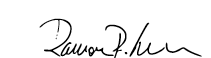
\includegraphics[width=65mm]{figs/logo/assinatura-ramon.png} \\[-4mm]
  \rule[2mm]{70mm}{0.1mm} \\
  \ramon \\[1mm]
  Coordenador do Projeto \\
}

%---------------------------------------------------------------------
\fim